%##################################################################################################

\chapter{Fundamentals}

%//////////////////////////////////////////////////////////////////////////////////////////////////

\section{Design Principles}

The main motivation behind the PLASMA project are performance shortcomings of \mbox{LAPACK}
and ScaLAPACK on shared memory systems, specifically systems consisting of multiple sockets
of multicore processors.
The three crucial elements that allow PLASMA to achieve performance greatly exceeding
that of LAPACK and ScaLAPACK are: the implementation of {\em tile algorithms}, the application
of {\em tile data layout} and the use of {\em dynamic scheduling}.
Although some performance benefits can be delivered by each one of these techniques
on its own, it is only the combination of all of them that delivers maximum performance
and highest hardware utilization.

%//////////////////////////////////////////////////////////

\subsection{Tile Algorithms}

Tile algorithms are based on the idea of processing the matrix by square tiles of relatively
small size, such that a tile fits entirely in one of the cache levels associated with one
core.
This way a tile can be loaded to the cache and processed completely before being evicted back
to the main memory.
Of the three types of cache misses, {\em compulsory}, {\em capacity} and {\em conflict},
the use of tile algorithms minimizes the number of capacity misses, since each operation
loads the amount of data that does not ``overflow'' the cache.

For some operations such as matrix multiplication and Cholesky factorization, translating
the classic algorithm to the tile algorithm is trivial.
In the case of matrix multiplication, the tile algorithm is simply a product of applying the
technique of {\em loop tiling} to the canonical definition of three nested loops.
It is very similar for the Cholesky factorization.
The \mbox{left-looking} definition of Cholesky factorization from LAPACK is a loop with
a sequence of calls to four routines: xSYRK (symmetric \mbox{rank-k} update), xPOTRF
(Cholesky factorization of a small block on the diagonal), xGEMM (matrix multiplication) and
xTRSM (triangular solve).
If the xSYRK, xGEMM and xTRSM operations are expressed with the canonical definition of three
nested loops and the technique of loop tiling is applied, the tile algorithm results.
Since the algorithm is produced by simple reordering of operations, neither the number of
operations nor numerical stability of the algorithm are affected.

The situation becomes slightly more complicated for LU and QR factorizations, where the
classic algorithms factorize an entire panel of the matrix (a block of columns) at every
step of the algorithm.
One can observe, however, that the process of matrix factorization is synonymous with introducing
zeros in approproate places and a tile algoritm can be fought of as one that zeroes one tile of
the matrix at a time.
This process is referred to as updating of a factorization or {\em incremental factorization}.
The process is equivalent to factorizing the top tile of a panel, then placing the upper
triangle of the result on top of the tile blow and factorizing again, then moving to the
next tile and so on.
Here, the tile LU and QR algorithms perform slightly more floating point operations and
require slightly more memory for auxiliary data.
Also, the tile LU factorization applies a different pivoting pattern and, as a result,
is less numerically stable than classic LU with full pivoting.
Numerical stability is not an issue in case of the tile QR, which relies on orthogonal
transformations (Householder reflections), which are numerically stable.

\begin{figure}[h!]
\centering
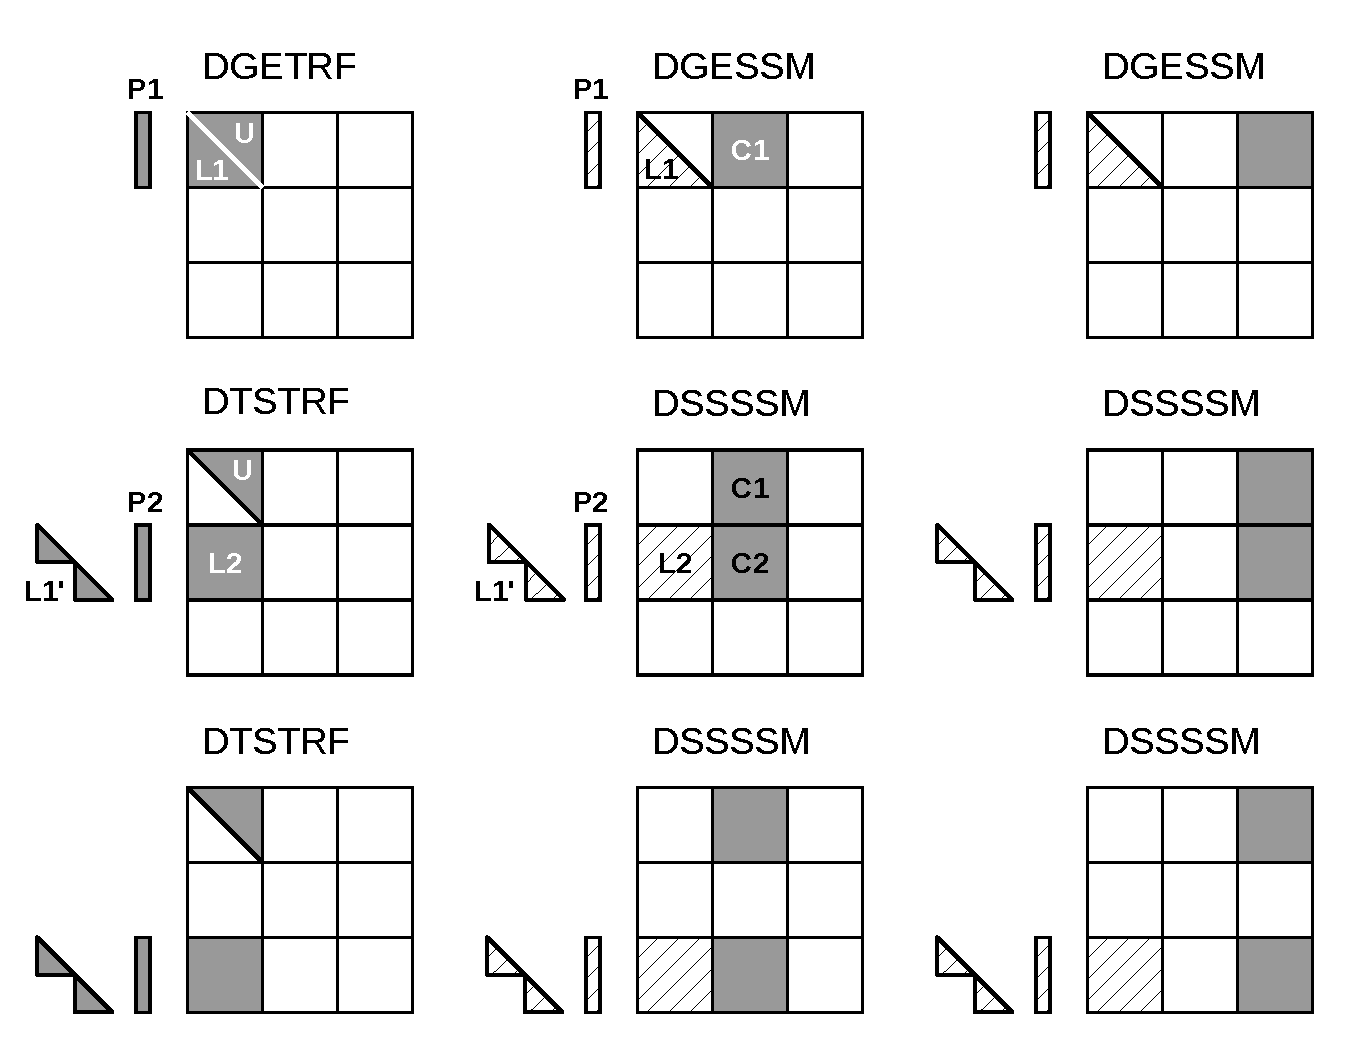
\includegraphics[width=0.60\columnwidth]{figures/tile_lu.pdf}
\caption{Schematic illustration of the tile LU factorization
         (kernel names for real arithmetics in double precision).}
\label{fig:tile_lu}
\end{figure}

%//////////////////////////////////////////////////////////

\subsection{Tile Data Layout}

Tile layout is based on the idea of storing the matrix by square tiles of relatively
small size, such that each tile occupies a continuous memory region.
This way a tile can be loaded to the cache memory efficiently and the risk of evicting it
from the cache memory before it is completely processed is minimized.
Of the three types of cache misses, {\em compulsory}, {\em capacity} and {\em conflict},
the use of tile layout minimizes the number of conflict misses, since a continuous region
of memory will completely fill out a \mbox{set-associative} cache memory before an eviction
can happen.
Also, from the standpoint of multithreaded execution, the probability of {\em false sharing}
is minimized. It can only affect the cache lines containing the beginning and the ending of a tile.

In standard \mbox{cache-based} architecture, tiles continously laid out in memory maximize
the profit from automatic prefetching.
Tile layout is also beneficial in situations involving the use of accelerators, where explicit
communication of tiles through DMA transfers is required, such as
moving tiles between the system memory and the local store in Cell B.~E. or moving tiles between
the host memory and the device memory in GPUs.
In most circumstances tile layout also minimizes the number of TLB misses and conflicts to memory
banks or partitions.
With the standard (\mbox{column-major}) layout, access to each column of a tile is much more likely
to cause a conflict miss, a false sharing miss, a TLB miss or a bank or partition conflict.
The use of the standard layout for dense matrix operations is a performance minefield.
Although occasionally one can pass through it unscathed, the risk of hitting a spot deadly to
performance is very high.

Another property of the layout utilized in PLASMA is that it is ``flat'', meaning that it does
not involve a level of indirection. Each tile stores a small square submatrix of the main matrix
in a \mbox{column-major} layout. In turn, the main matrix is an arrangement of tiles immediately
following one another in a \mbox{column-major} layout.
The offset of each tile can be calculated through address arithmetics and does not involve pointer
indirection.
Alternatively, a matrix could be represented as an array of pointers to tiles, located anywhere
in memory. Such layout would be a radical and unjustifiable departure from LAPACK and ScaLAPACK.
Flat tile layout is a natural progression from LAPACK's \mbox{column-major} layout and ScaLAPACK's
\mbox{block-cyclic} layout.

Another related property of PLASMA's tile layout is that it includes provisions for padding of tiles,
i.e., the actual region of memory designated for a tile can be larger than the memory occupied by
the actual data.
This allows to force a certain alignment of tile boundaries, while using the flat organization
described in the previous paragraph.
The motivation is that, at the price of small memory overhead, alignment of tile boundaries may
prove benefivial in multiple scenarios involving memory systems of standard multicore processors,
as well as accelerators.
The issues that come into play are, again, the use of TLBs and memory banks or partitions.

\begin{SCfigure}
\centering
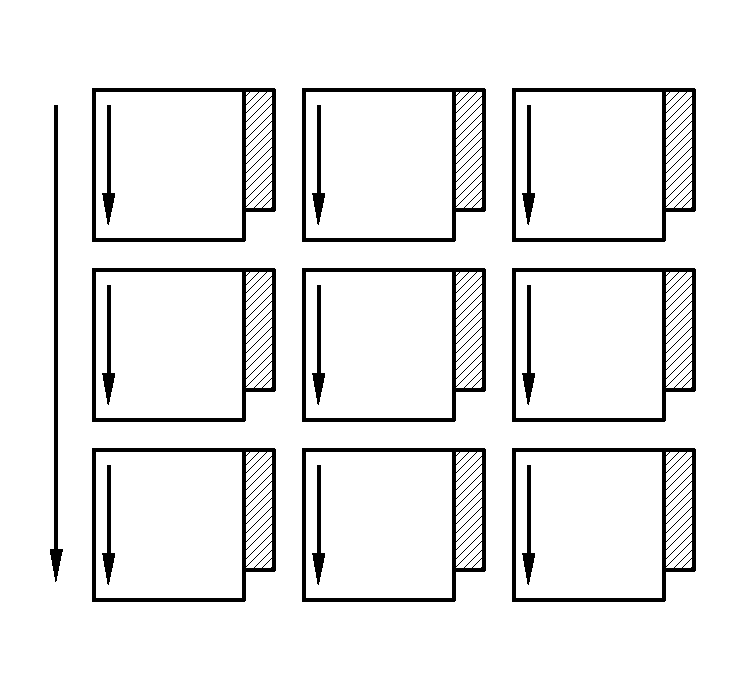
\includegraphics[width=0.5\columnwidth]{figures/tile_layout.pdf}
\caption{Schematic illustration of the tile layout with \mbox{column-major}
         order of tiles, \mbox{column-major} order of elements within tiles
         and (optional) padding for enforcing a certain alighment of tile bondaries.}
\label{fig:tile_layout}
\end{SCfigure}

%//////////////////////////////////////////////////////////

\subsection{Dynamic Task Scheduling}

Dynamic scheduling is the idea of assigning work to cores based on the availability of data
for processing at any given point in time and is also referred to as \mbox{\em data-driven}
scheduling.
The concept is related closely to the idea of expressing computation through a task graph,
often referred to as the DAG ({\em Direct Acyclic Graph}), and the flexibility exploring
the DAG at runtime.
Thus, to a large extent, dynamic scheduling is synonymous with \mbox{\em runtime scheduling}.
An important concept here is the one of the {\em critical path}, which defines the upper bound
on the achievable parallelism, and needs to be pursued at the maximum speed.
This is in direct opposition to the \mbox{\em fork-and-join} or \mbox{\em data-parallel}
programming models, where artificial synchronization points expose serial sections of
the code, where multiple cores are idle, while sequential processing takes place.
The use of dynamic scheduling introduces a \mbox{trade-off}, though.
The more dynamic (flexible) scheduling is, the more centralized (and less scalable)
the scheduling mechanism is.
For that reason, currently PLASMA uses two scheduling mechanisms, one which is fully dynamic
and one where work is assigned statically and dependency checks are done at runtime.

The first scheduling mechanism relies on unfolding a {\em sliding window} of the task graph
at runtime and scheduling work by resolving data hazards: {\em Read After Write~(RAW)},
{\em Write After Read~(WAR)} and {\em Write After Write~(WAW)}, a techniqe analogous
to instruction scheduling in superscalar processors.
It also relies on \mbox{\em work-stealing} for balanding the load among all multiple cores.
The second scheduling mechanism relies on statically designating a path through the execution
space of the algorithm to each core and following a cycle: transition to a task, wait for its
dependencies, execute it, update the overall progress.
Task are identified by tuples and task transitions are done through locally evaluated formulas.
Progress information can be centralized, replicated or distributed (currently centralized).

\begin{figure}[h!]
\centering
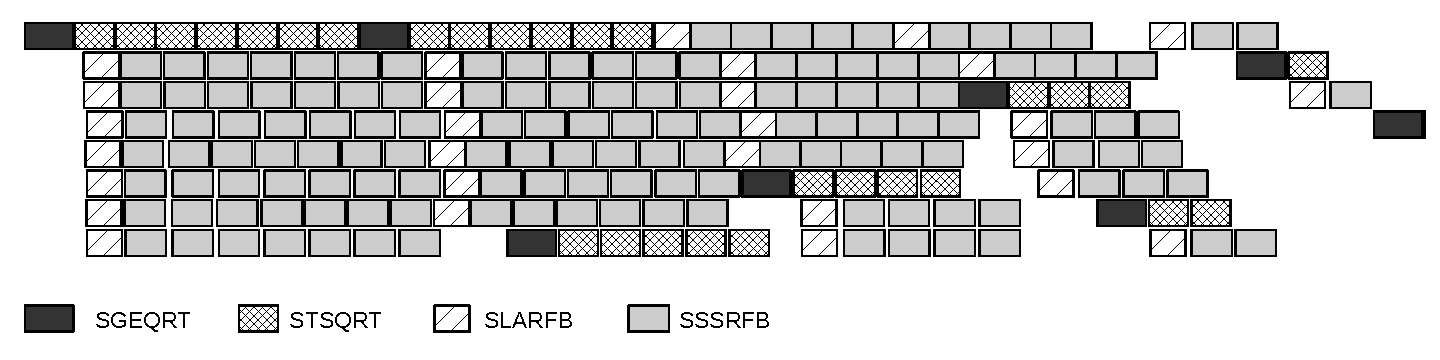
\includegraphics[width=0.8\columnwidth]{figures/trace_qr.pdf}
\caption{A trace of the tile QR factorization executing on eight cores
         without any global synchronization points
         (kernel names for real arithmetics in single precision).}
\label{fig:cholesky_trace}
\end{figure}

%//////////////////////////////////////////////////////////////////////////////////////////////////

\section{Software Stack}

Starting from the PLASMA Version 2.2, release in July 2010, the library is built on top of standard
software components, all of which are either available as open source or are standard OS facilities.
Some of them can be replaced by packages provided by hardware vendors for efficiency reasons.
Figure~\ref{fig:software_stack} presents the current structure of PLASMA's software stack.
Following is the \mbox{bottom-up} description of individual components.

\begin{figure}[h!]
\centering
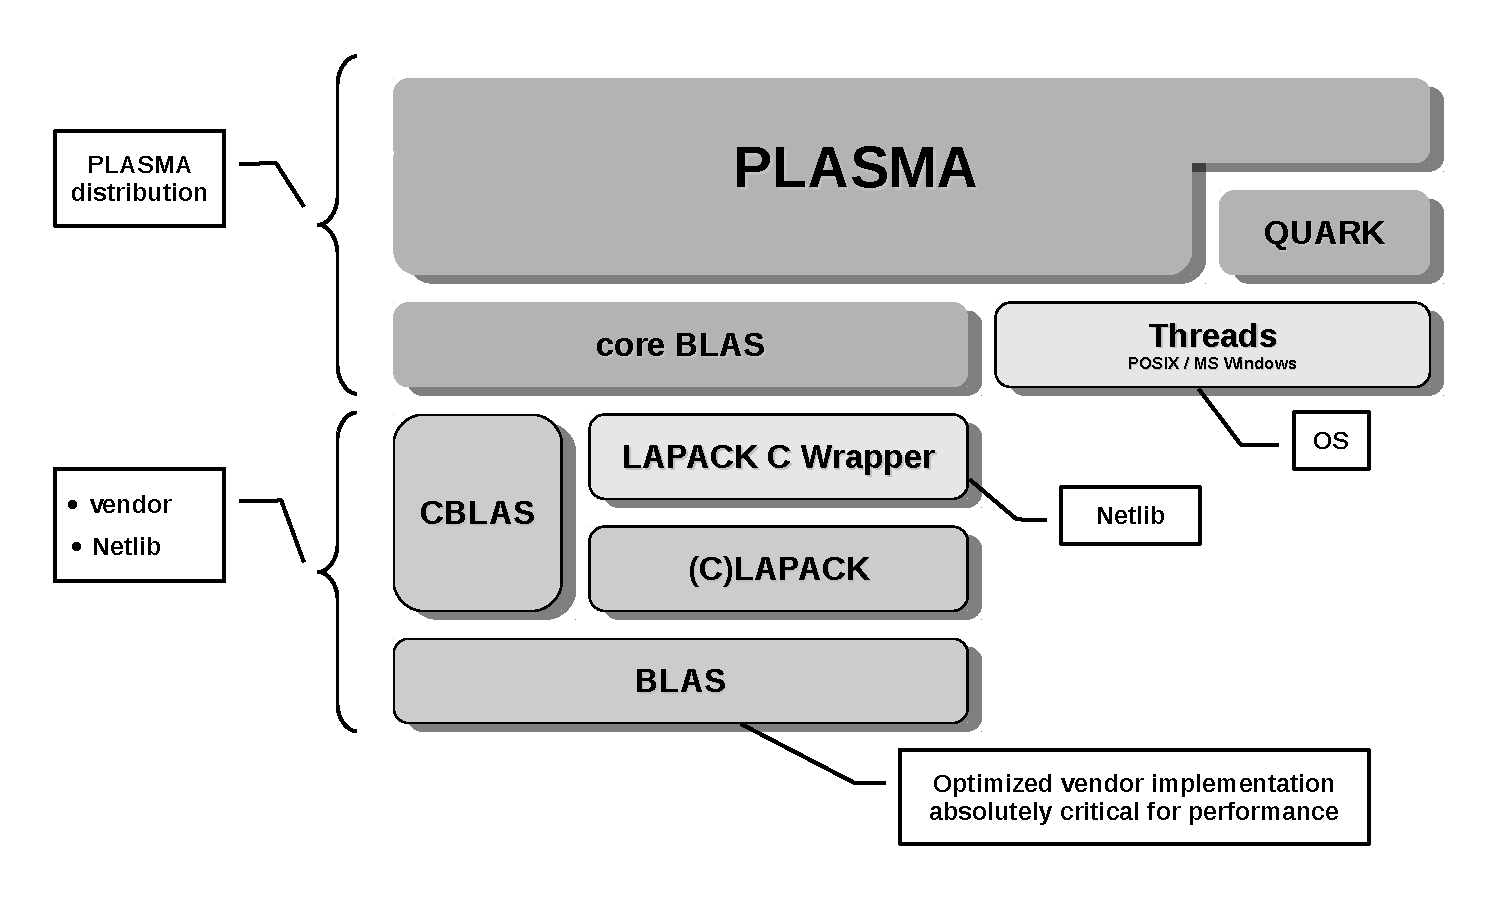
\includegraphics[width=0.8\columnwidth]{figures/software_stack.pdf}
\caption{The software stack of PLASMA Version 2.3.}
\label{fig:software_stack}
\end{figure}

\begin{description}
\item[BLAS]
is a set of Basic Linear Algebra Subprograms, a {\em de facto} standard for basic linear algebra
operations such as vector and matrix multiplication.
The definition of BLAS is available from Netlib in the form of unoptimized FORTRAN code.
Highly optimized implementations are available from many hardware vendors, such as Intel and AMD.
Fast implementations are also available in the form of academic packages, such as Goto BLAS
and ATLAS.
The standard interface to BLAS is the FORTRAN interface.

\item[CBLAS]
is the C language interface to BLAS.
The definition of CBLAS is available from Netlib in the form of a set of C wrappers for BLAS
with FORTRAN interface. Most commercial and academic implementations of BLAS also provide CBLAS.
Most people refer to CBLAS as a thin C language interoperability layer on top of an actual
implementation available through a FORTRAN interface.

\item[LAPACK]
(Linear Algebra PACKage) is a software library for numerical linear algebra, a direct predecessor
of PLASMA, providing routines for solving linear systems of equations, linear least square problems,
eigenvalue problems and singular value problems.
Many commercial and academic implementations of BLAS include a small subset of most common LAPACK
routines, such as LU, Cholesky and QR factorizations.
PLASMA uses a subset of LAPACK routines commonly provided with BLAS.

CLAPACK is a version of LAPACK available from Netlib created by automatically translating FORTRAN
LAPACK to C with the help of the F2C utility.
It provides LAPACK functionality in situations when only a C compiler is available.
At the same time, it provides the same calling convention as the ``original'' LAPACK,
the FORTRAN interface that conforms, for the most part, to the GNU g77 Application Binary
Interface~(ABI).

\item[LAPACK C Wrapper]
is a C language interface to LAPACK (or CLAPACK).
While at the time of writting this guide the effort is underway to standardize the C interface
to LAPACK, it has not been finalized yet.
For the time being, an implementation of the C interface is provided by Netlib.
Since it has not been standardized yet, it is not available from any other source.

\item[core BLAS]
is a set of serial kernels, the building blocks for PLASMA algorithms.
Ideally, core BLAS would be imlemented as monolythic kernels that are carefully optimized
for a given architecture.
This amounts, however, to a prohibitive coding effort mainly due the challenges of SIMD'zation
for vector extensions ubiquitous in modern processors.
Instead, these kernels are currently constructed from calls to BLAS and LAPACK, which is a suboptimal
way of implementing them, but the only feasible one known to the authors.

\item[Threads]
are the main mechanism for parallelization in PLASMA.
Currently relies on basic threading facilities such as launching and merging of threads,
mutexes and conditional variables.
Currently PLASMA natively supports POSIX threads and Microsoft Windows threads.

\item[QUARK]
is a simple dynamic scheduler provided with the PLASMA distribution, similar in desing principles
to the Jade project from the Massachusetts Institute of Technology, the SMPSs system from the
Barcelona Supercomputer Center, and the StarPU system from INRIA Bordeaux.
While sharing multiple slimilarities with the other projects, QUARK provides a number of extensions
necessary for integration with a numerical library such as PLASMA.
Besides serving as a component of PLASMA, QUARK is a \mbox{stand-alone} scheduler and can be
easily used outside of PLASMA.

\end{description}

One can observe that while
CBLAS provides the C interface to BLAS without the actual implementation,
CLAPACK provides the implementation of LAPACK without the actual C interface.

%//////////////////////////////////////////////////////////////////////////////////////////////////




%##################################################################################################
